% Opcje klasy 'iithesis' opisane sa w komentarzach w pliku klasy. Za ich pomoca
% ustawia sie przede wszystkim jezyk oraz rodzaj (lic/inz/mgr) pracy.
\documentclass[shortabstract]{iithesis}

\usepackage[utf8]{inputenc}
\usepackage{graphicx} % Required for including images
\graphicspath{ {.} }
\usepackage[font=small,labelfont=bf]{caption}

%%%%% DANE DO STRONY TYTUŁOWEJ
% Niezaleznie od jezyka pracy wybranego w opcjach klasy, tytul i streszczenie
% pracy nalezy podac zarowno w jezyku polskim, jak i angielskim.
% Pamietaj o madrym (zgodnym z logicznym rozbiorem zdania oraz estetyka) recznym
% zlamaniu wierszy w temacie pracy, zwlaszcza tego w jezyku pracy. Uzyj do tego
% polecenia \fmlinebreak.
\polishtitle    {Raspberry Pi BASIC}
\englishtitle   {}
\polishabstract {Celem niniejszej pracy jest implementacja systemu z interpreterem języka programowania BASIC działającego na mikrokomputerah z serii Raspberry Pi w wersji 3. i 4. Zaproponowany dialekt bazuje na tym wykorzystywanym w latach '80 w popularnych komputerach Commodore 64. Program nie tylko umożliwia pracę w starym stylu na współczesnym sprzęcie, ale także prezentuje możliwości jakie dają te popularne płytki i pokazuje jak wykorzystać je programując bare metal, co stanowi większe wyzwanie niż w przypadku gdy jest ona kontrolowana przez dedykowany system operacyjny Raspbian. Wykorzystując wbudowane złącza projekt wspiera obsługę karty SD oraz wyjście wideo HDMI, a także poprzez wyprowadzone piny GPIO umożliwia podłączenie zewnętrznej klawiatury ze złączem PS2 lub DIN5.}
\englishabstract{The aim of this thesis is to implement a system with a BASIC programming language interpreter that runs on Raspberry Pi series microcomputers versions 3. and 4. The proposed dialect is based on the one used in the '80s in the popular Commodore 64 computers. The program not only allows retro-style operation on modern hardware, but also demonstrates the capabilities of these popular boards. In addition, it presents how to take advantage of the Raspberry Pi's features by programming bare-metal, which is rather more demanding than when managed by a dedicated Raspbian operating system. Using the built-in connectors, the project provides support for SD card and HDMI video output, along with the ability to connect an external keyboard with a PS2 or DIN5 port through the derived GPIO pins.}
% w pracach wielu autorow nazwiska mozna oddzielic poleceniem \and
\author         {Aleksandra Kosińska \and Cezary Stajszczyk}
% w przypadku kilku promotorow, lub koniecznosci podania ich afiliacji, linie
% w ponizszym poleceniu mozna zlamac poleceniem \fmlinebreak
\advisor        {dr Piotr Polesiuk}
\date           {31 sierpnia 2023}                     % Data zlozenia pracy
% Dane do oswiadczenia o autorskim wykonaniu
\transcriptnum {317341 \and 317354}                     % Numer indeksu
\advisorgen    {dr. Piotra Polesiuka} % Nazwisko promotora w dopelniaczu
%%%%%

%%%%% WLASNE DODATKOWE PAKIETY
%
%\usepackage{graphicx,listings,amsmath,amssymb,amsthm,amsfonts,tikz}
%
%%%%% WŁASNE DEFINICJE I POLECENIA
%
%\theoremstyle{definition} \newtheorem{definition}{Definition}[chapter]
%\theoremstyle{remark} \newtheorem{remark}[definition]{Observation}
%\theoremstyle{plain} \newtheorem{theorem}[definition]{Theorem}
%\theoremstyle{plain} \newtheorem{lemma}[definition]{Lemma}
%\renewcommand \qedsymbol {\ensuremath{\square}}
% ...
%%%%%

\begin{document}

%%%%% POCZĄTEK ZASADNICZEGO TEKSTU PRACY

\chapter{Wstęp}
Dynamiczne tempo rozwoju w dziedzinie informatyki prowadzi do powstawania nowoczesnych technologii oraz narzędzi programistycznych. Niemniej jednak, fundamentalne zrozumienie działania systemów komputerowych na jak najniższej warstwie abstrakcji zachowuje swoją edukacyjną i badawczą wartość.
Celem niniejszej pracy inżynierskiej jest zaprojektowanie oraz implementacja systemu operacyjnego działającego w środowisku bare-metal na platformie RaspberryPi, umożliwiającego tworzenie i uruchamianie programów napisanych w języku BASIC. Zainteresowanie programowaniem niskopoziomowym, systemami wbudowanymi oraz retroinformatyką wpłynęło na wybór tematu pracy.
Przyjęty temat pracy umożliwia pogłębienie wiedzy w zakresie zarządzania sprzętem w środowisku pozbawionym klasycznego systemu operacyjnego oraz analizę wyzwań związanych z implementacją interpretera języka programowania na takim systemie.


\chapter{Podstawy projektu}
Raspberry Pi to nazwa serii komputerów jednopłytkowych stworzonych przez brytyjską organizację charytatywną, której celem jest edukowanie ludzi w zakresie informatyki i ułatwianie dostępu do edukacji informatycznej. Oryginalnie Raspberry Pi zostało wyprodukowane z myślą o języku Python, jednak w prezentowanej pracy obrano zupełnie inne podejście do użytkowania tego urządzenia. Skupiono się na programowaniu niskopoziomowym - tworząc kod w języku C i Asembler który działa na sprzęcie bezpośrednio, bez żadnej podstawowej abstrakcji, takiej jak system operacyjny.

\section{Budowa projektu}
\section{GPIO}
\begingroup
\centering
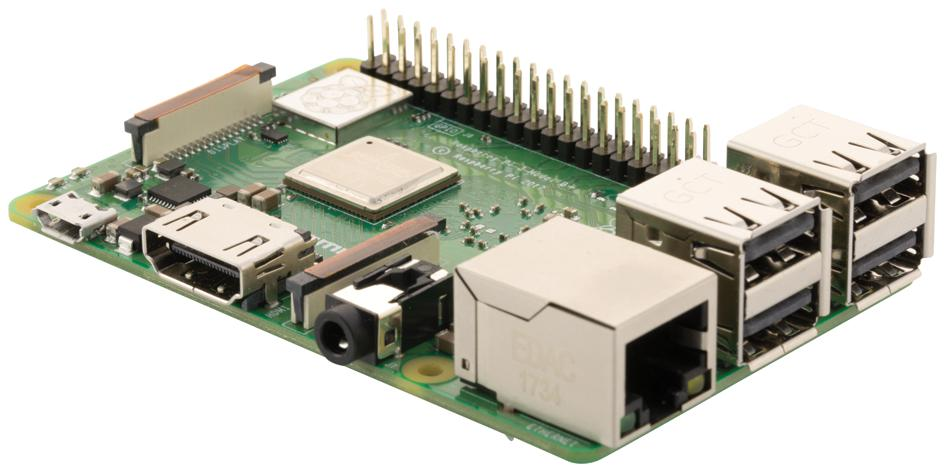
\includegraphics[width=0.75\textwidth]{rpi3b.jpg}
\captionsetup{type=figure}
\caption{Płytka Raspberry Pi 3B}
\endgroup
Programowanie systemów wbudowanych, stanowi wyjątkowe wyzwanie inżynieryjne. Charakter tego typu projektów wymaga nie tylko zaawansowanej wiedzy technicznej, ale również wykorzystania odpowiednich narzędzi, które uwzględniają specyfikę docelowej platformy sprzętowej. Przy niewłaściwym podejściu istnieje ryzyko, że RaspberryPi nie uruchomi się w sposób zamierzony. W niniejszym rozdziale przedstawiona zostanie struktura oraz proces konstrukcji projektu systemu niskopoziomowego przeznaczonego dla platformy RaspberryPi.
\subsection{Cross-compiler}
W ramach projektowania systemów niskopoziomowych dla specyficznych platform, takich jak RaspberryPi, kluczowym narzędziem jest cross-compiler (kompilator skrośny). Ze wzgędu na to, że architektura procesorów RaspberryPi różni się od konwencjonalnych komputerów, kompilacja bezpośrednio na nich byłaby nieefektywna. Cross-compiler, jak nazwa wskazuje, pozwala kompilować kod na jednej platformie tak, aby był on przeznaczony do wykonania na innej. W niniejszym projekcie, jako kompilator skrośny został wykorzystany \texttt{aarch64-linux-gnu}, który jest dedykowany dla architektury ARM.
\subsection{Struktura katalogów}
Projekt jest zorganizowany w przejrzystą strukturę katalogów. Katalog \texttt{src} zawiera pliki źródłowe z rozszerzeniem \texttt{.c} i \texttt{.S}, definiujące logiczną strukturę projektu. Natomiast, katalog \texttt{include} gromadzi pliki nagłówkowe \texttt{.h}, które umożliwiają deklaracje funkcji, struktur danych oraz innych kluczowych elementów używanych w kodzie źródłowym.
\subsection{Proces budowy}
Ważnym elementem każdego projektu programistycznego jest automatyzacja procesu budowy. W tym celu zostało wykorzystane narzędzie \texttt{Makefile}. Za jego pośrednictwem pliki źródłowe są kompilowane w kolejności, następnie łączone, tworząc finalny plik wykonywalny w formacie \texttt{.elf}. Zastosowanie narzędzia \texttt{objcopy} umożliwia transformację tego pliku do końcowego obrazu systemu \texttt{kernel8.img}.
Linkowanie to proces łączenia plików obiektowych oraz bibliotek w jednolitą całość, składającą się na plik wykonywalny. W przedstawionym projekcie jest to kluczowy krok, który pozwala na właściwe zorganizowanie segmentów pamięci, zapewnienie poprawnych odwołań do funkcji oraz właściwą inicjalizację systemu.
\subsection{Armstub}
W \texttt{Makefile}, oprócz zdefiniowanych procedur kompilacji, zawarte są również instrukcje dotyczące tworzenia \texttt{armstub}'a. W tym projekcie odgrywwa on niezwykle istotną rolę. Jest to składnik, który pozwala na zapewnienie kompatybilności między różnymi wersjami RaspberryPi. Dzięki użyciu własnego \texttt{armstub}'a, możliwe jest ujednolicenie procesu bootowania niezależnie od specyfikacji sprzętowej poszczególnych wersji platformy.

\section{Przygotowanie karty pamięci}
Aby Raspberry Pi mogło uruchomić napisany program należy najpierw odpowiednio przygotować kartę pamięci. Pierwszy wpis w MBR musi wskazywać na partycję typu FAT16 lub FAT32. Jej zalecany przez producenta to 256MB. Do samego uruchomienia komputera ta jedna partycja jest wystarczająca, ale na potrzeby tego projektu rekomendowane jest utworzenie drugiej partycji do przechowywania danych, jednak to bedzie bardziej szczegółowo opisane w jednym z kolejnych rozdziałów. W internecie można znaleźć listy kompatybilnych kart, jednak producent nie wydał żadnych oficjalnych rekomendacji co do wspieranych typów. W praktycje jednak zdecydowana więszkość kart nadaje się do pracy z Raspberry Pi.
\subsection{Niezbędne pliki}
Gdy karta SD jest już odpowiednio sformatowana, należy na partycji odpowiedzialnej za bootowanie umieścić odpowiednie pliki:
\begin{itemize}
 \item \texttt{config.txt}  - Plik z początkową konfiguracją płytki czytany przez bootloader. W komputerach domowych taka początkowa konfiguracja jest zazwyczaj przechowywana w pamięci BIOSu. Raspberry Pi jednak go nie posiada, dlatego konfiguracaj przechowywana jest w zwyczajnym pliku tekstowym.
 \item \texttt{bootcode.bin}  - Zawiara kod bootloadera. Wykonuje on podstawową konfiguracje, a następnie ładuje plik \texttt{start.elf}. Jest wymagany tylko na RPi3, w nowszych wersjach płytki został zastąpiony przez kod zapisany w pamięci EEPROM bezpośrednio na płytce. Można go pozyskać z instalacji zwykłego Raspbiana dostępnego na stronie producenta.
 \item \texttt{start.elf}  - Kod z firmwarem, odpowiedzialny za uruchomienie GPU oraz przeczytanie i wdrożenie konfiguracji z pliku \texttt{config.txt}. Również dostępny z Raspbianem.
 \item \texttt{kernel8.img}  - Najważniejszy plik zawierający cały kod projektu. Ósemka na końcu nazwy oznacza, że jest to obraz 64-bitowy. Zostanie on domyślnie załadowany pod adres 0x80000 (512KB)
 \item \texttt{armstub.bin}  - Ten plik w ogólności nie jest niezbędny do uruchomienia mikrokomputera, ale jest szczególnie istotny z perspektywy tego projektu, ponieważ w założeniu projekt ma działać na Rasperry Pi zarówno w wersji 3. jak i 4. Jest to dodatkowa część bootloadera ładowana pod adres 0x0, która wykonywana jest przed kodem z kernel8.img i ma na celu ujednolicenie stanu maszyny przed przejściem do kodu głównego, ponieważ domyślnie różne wersje płytek bootują się z nieco innymi konfiguracjami.
\end{itemize}

\section{Bootowanie}
Bootowanie systemów wbudowanych, takich jak RaspberryPi, to kluczowy proces inicjalizacji, który determinuje, czy system zostanie poprawnie załadowany i uruchomiony. Każdy element tego procesu odgrywa istotną rolę w zapewnieniu właściwej funkcji urządzenia.
\subsection{Funkcja pliku config.txt}
Pierwszym istotnym elementem procesu bootowania jest plik \texttt{config.txt}. W tym pliku zawarte są kluczowe informacje konfiguracyjne dla bootloadera, które otrzymuje podczas startu systemu. Umożliwia on określenie parametrów takich jak np. częstotliwość taktowania zegara. 
\subsection{Proces bootowania RaspberryPi}
Proces bootowania RaspberryPi rozpoczyna się od wczytania z karty SD pliku \texttt{bootcode.bin}, który jest odpowiedzialny za inicjalizację podstawowych komponentów układu. Następnie, wczytywany jest plik systemowy \texttt{start.elf}, który pełni rolę bootloadera. Gdy proces bootowania osiągnie etap ładowania \texttt{kernel8.img}, rozpoczyna się wykonywanie kodu zawartego na początku tego pliku. W przypadku przedstawionego projektu, jest to kod źródłowy pochodzący z \texttt{boot.S}. Ten fragment kodu Asemblera odpowiada za inicjalizację kluczowych elementów systemu, takich jak ustawienie odpowiedniego poziomu wyjątku, aktywacja jednostki Floating-Point Unit oraz dezaktywacja nieużywanych rdzeni procesora. Jego rozmieszczenie na początku obrazu jest gwarantowane przez instrukcje zawarte w pliku \texttt{linker.ld}. Po pomyślnym przejściu przez te wstępne operacje, kontrola jest przekazywana do funkcji \texttt{main()}.
\subsection{Sygnalizacja statusu bootowania za pomocą LED}
Wbudowany mechanizm diagnostyczny RaspberryPi pozwala na szybką identyfikację problemów występujących w trakcie bootowania. Sygnalizacja odbywa się za pomocą zintegrowanej zielonej diody LED na płytce RaspberryPi. Znaczenie poszczególnych sekwencji mrugnięć jest następujące:
\begin{itemize}
 \item ciągłe światło - wskazuje, że karta SD została prawidłowo podłączona;
 \item szybkie mruganie - oznacza aktywny odczyt lub zapis na kartę SD;
 \item trzy mrugnięcia - sygnalizują niepowodzenie procesu bootowania;
 \item cztery mrugnięcia - informują o braku pliku \texttt{start.elf na karcie SD};
 \item siedem mrugnięć - wskazują na brak pliku \texttt{kernel.img};
 \item osiem lub dziewięć mrugnięć - sygnalizują błąd pamięci SDRAM;
 \item dziesięć mrugnięć - stan "halt", wskazujący na krytyczny błąd systemu.
\end{itemize}

\section{Debugowanie}
W środowisku embedded, diagnozowanie oraz wykrywanie błędów jest procesem niezwykle skomplikowanym ze względu na bezpośrednią interakcję napisanego systemu z warstwą sprzętową. Kolejnym utrudnieniem jest brak wsparcia rozbudowanych mechanizmów diagnostycznych, które dostępne są w pełnych systemach operacyjnych. 
\subsection{Mechanizmy obsługi przerwań i wyjątków}
W omawianym projekcie, podczas inicjalizacji systemu ustawiany jest poziom uprzywilejowania dostępu na Exception Level 1. Mechanizmy przerwań stanowią kluczowy element w systemach bare-metal, umożliwiając skuteczną komunikację i reakcję na specyficzne zdarzenia generowane przez komponenty sprzętowe. Odpowiedno skonfigurowane procedury pozwalają na obsługę przerwań, które są oczekiwane. 
Sytuacje nieprzewidziane, które również mogą wystąpić, prowadzą do generowania przerwań niespodziewanych. W takim wypadku, procedura diagnostyczna systemu reaguje poprzez wyświetlenie identyfikatora danego przerwania oraz wartości zawartych w rejestrach \texttt{elr\_el1} oraz \texttt{esr\_el1}. Rejestr \texttt{elr\_el1}, będący skrótem od "Exception Link Register", przechowuje adres powrotu po zakończeniu obsługi wyjątku. Z kolei \texttt{esr\_el1} (Exception Syndrome Register) zawiera informacje na temat przyczyn wystąpienia konkretnego zdarzenia. Dzięki interpretacji danych z tych rejestrów, możliwe jest precyzyjne zidentyfikowanie i rozwiązanie źródła problemu.
\subsection{Deasemblacja}
Plik Makefile zawiera polecenie, które umożliwia generowanie zdezasemblerowanego obrazu pliku .elf. Wykorzystując komendę \texttt{aarch64-linux-gnu-objdump -D ./build/kernel8.elf > code.txt} uzyskujemy przetworzony kod do formy tekstowej, reprezentującej sekwencje instrukcji asemblerowych.


\chapter{BASIC}
BASIC to język, a w zasadzia cała rodzina języków programowania, której historia zaczyna się w 1963 roku (w Dartmouth College. Twórcami oryginalnej wersji byli John G. Kemeny oraz Thomas E. Kurtz). Na przestrzeni 60 lat pojawiło się wiele dialektów tego języka, jednak ich ogólne założenia, składnia i zbiór instrukcji były do siebie bardzo zblizone. Dialekt zaproponowany w tej pracy bazuje na tym wykorzystywanym w popularnych komputeraz Commodore 64, jednak nie jest jego dokładnym odwzorowaniem.

\begin{verbatim}
10 PRINT "FIBONACCI"
20 INPUT "N?" N
30 DIM TAB[N]
40 LET TAB[0] = 1 : TAB[1] = 1
50 FOR I=2 TO N-1
60 LET TAB[I] = TAB[I-1] + TAB[I-2]
70 NEXT
80 PRINT "FIB(";N;")=";TAB[N-1]
90 END
\end{verbatim}

Programy pisze się inaczej niż jakby robiło się to w zwykłym edytorze tekstu. Każdą instrukcję poprzedza się odpowiadającym jej numerem linii. Zwyczajowo instrukcje numeruje się kolejnymi wielokrotnościami liczby 10, aby pozostawić miejsce na dodawanie nowych instrukcji pomiędzy już istniejące. Dodanie instrukcji o już istniejącym numerze ją nadpisuje. Moduły odpowiedzialne za obsługę BASICa zostały bardziej szczegółowo opisane w następnych podrozdziałach.

\section{Sesja}
W wielu językach programowania, organizacja i zarządzanie danymi są kluczem do skutecznej i efektywnej egzekucji programu. W przedstawionym projekcie wprowadzony został moduł o nazwie “Session”, który pełni znaczącą rolę w tym zakresie. Jest on odpowiedzialny nie tylko za przechowywanie wszystkich danych związanych z programem ale również za trzymanie informacji o aktualnym stanie wykonywania programu i ewentualnych kodach błędu. Ponadto jego rolą jest prawidłowe przekazywanie zapisanych instrukcji do interpretera zważając na ich kolejność oraz potencjalne skoki. Funkcjonowanie modułu ma bezpośredni wpływ na zdolność użytkownika do pisania, uruchamiania czy modyfikowania programów w języku BASIC. W związku z tym, moduł "Session" jest jednym z najważniejszych elementów w części systemu, która obsługuje interpretację języka programowania BASIC.
\subsection{Struktury Modułu Session}
Głównym elementem modułu "Session" jest struktura \texttt{sessionS}. Została ona zdefiniowana następująco:
\begin{verbatim}
typedef struct sessionS {
  metadataS metadata;
  forS for_stack[8];
  u64 return_address_stack[32];
  dataQueueS data_queue[128];
  variableS variables[64];
  functionS functions[64];
} sessionS;
\end{verbatim}

Język BASIC udostępnia instrukcje, które mogą skakać do wyznaczonych linii programu, dlatego potrzebny jest stos adresów powrotu, który wykorzystany został do zapamiętywania numerów linii w celu prawidłowej kolejności wykonania programu. Kolejnym z komponentów jest kolejka danych, z której użytkownik może ściągać i odkładać zmienne za pomocą dedykowanych instrukcji. W środowisku sesji znajdują się również zapisane funkcje oraz zmienne, które w swoich strukturach oprócz wartości przechowują zdefiniowane w programie nazwy, aby można się było do nich odwołać. Kluczowym elementem są metadane, które zawierają wskaźniki umożliwiające edytowanie oraz poruszanie się po liście instrukcji. Struktura \texttt{metadataS} zawiera również informacje o bieżącym stanie sesji, występującym kodzie błędu (znacząco ułatwia obsługę i diagnostykę problemów) oraz szczegółowe informacje podstruktur \texttt{sessionS} (np. liczba zmiennych). Ważnym elementem jest flaga skoku, której celem jest poinformowanie modułu o ewentualnej zmianie kolejności wykonywanych instrukcji. Metadane te są niezbędne dla wielu funkcji zawartych w tym module, umożliwiając im prawidłowe działanie.
Instrukcje programu są przechowywane w formie listy dwukierunkowej. Każdy węzeł tej listy, oprócz wskaźników na następny i poprzedni węzeł, przechowuje również numer linii oraz treść instrukcji jako ciąg znaków.
\subsection{Operacje na strukturze sessionS}
Zarządzanie sesją w opisywanym module nie ogranicza się wyłącznie do przechowywania danych. Zawiera on również różnego rodzaju funkcje, które umożliwiają efektywne operowanie na tej strukturze. Funkcje w "Session" dają możliwość dodawania, modyfikowania i usuwania elementów takich jak: zmienne, funkcje oraz instrukcje. Umożliwiają także przeprowadzanie operacji na kolejce danych zgodnie z wymaganiami języka BASIC. Co więcej, moduł pozwala na uruchomienie całego programu, co jest jego najważniejszą czynnością. Ostatecznie wszystkie operacje dostępne w module tworzą pełny zestaw fundamentów, niezbędny do przetwarzania i wykonywania kodu w języku BASIC. Dzięki temu użytkownik może w pełni korzystać z możliwości interpretera, mając pewność, że każda operacja jest przeprowadzana w sposób prawidłowy.

\section{Parser}
  Moduł parsera jest zdecydowanie mniejsze i prostszy od pozostałych. Jego główna funkcja \texttt{get\_next\_token()} ma za zadanie dla podanego ciągu znaków zwrócić ID tokenu występującego na początku i przesunięcie wskaźnika za przeczytany token. W przypadku niektórych tokenów (na przykład liczby lub nazwy zmiennych) oprócz ID  tokenu niezbędna jest również znajomość jego dokładnej wartości, dlatego przeczytany ciąg znaków jest kopiowany do bufora podanego jako argument funkcji. Kolejność sprawdzania tokenów jest następująca: znak końca linii, liczby (również te w formacie szesnastkowym), słowa kluczowe i operatory, a na końcu nazwy zmiennych i funkcji. Kolejność ta powoduje, że stworzenie zmiennej o nazwie będącej słowem kluczowym jest niemożliwe - parser nigdy nie rozpozna tego jako nazwę zmiennej. Parser ma również wbudowaną funkcjonalność zgłaszania błędów - gdy użytkownik wie, jakiego konkretnego tokenu się spodziewa, może podać jego ID jako argument funkcji. Jeżeli odnaleziony token nie będzie pasować, parser sam zgłosi błąd.

\section{Interpreter}
  Zadaniem interpretera jest wykonanie instrukcji na podstawie ciągu tokenów zwracanych mu przez parser. Skutkiem wykonania instrukcji mogą być dwie rzeczy: zmiana struktury sesji (zdecydowana większość przypadków) lub wydrukowanie czegoś na ekranie (na przykład z pomocą instrukcji \texttt{PRINT}, ale mogą to też być informacje o błędach). Do wykonania każdej z dostępnych instrukcji napisana została osobna funkcja. Konstrukcja BASICa jest na tyle prosta, że już po pierwszym przeczytanym tokenie wiadomo jakiej instrukcji sie spodziewać. Główna funkcja czyta pierwszy token, a następnie na jego podstawie wybiera odpowiednią funkcję i przekazuje jej ciąg znaków będący pozostałą częścią instrukcji.
\subsection{Tryb bezpośredni}
Oprócz możliwości pisania całych programów możliwe jest również wykonywanie instrukcji w tak zwanym trycie bezpośrednim. Instrukcja wpisana w trybie bezpośrednim poznawana jest po tym, że nie jest poprzedzona numerem linii. Taka instrukcja nie jest nigdzie zapisywana, a jest wykonywana od razu. Daje możliwość na przykład opowiedniego przygotowania środowiska przed uruchomieniem programu i jest niezwykle przydatne podczas debugowania. W dowolnym momencie programu można się zatrzymać instrukcją \texttt{STOP}, a następnie przeprowadzić inspekcję w trybie bezpośrednim, skorygować ewentualne błędy i wznowić działanie programu wpisując \texttt{CONT}. Niektóre instrukcje (takie jak właśnie \texttt{CONT} lub \texttt{RUN}) można wpisywać tylko w trybie bezpośrednim.

\section{Ewaluator}
Język BASIC dopuszcza używanie wyrażeń arytmetyczno-logicznych jako argument słów kluczowych. Oznacza to, że tak jak w większości innych języków programowania, możemy np. zdefiniować zmienną za pomocą działania arytmetycznego (\texttt{LET x = 1+1}). Z tego powodu w projekcie potrzebny jest moduł odpowiedzialny za obliczanie wartości wyrażeń.
\subsection{Algorytm ewaluacji wyrażeń}
Evaluator jako jeden z argumentów - w postaci ciągu znaków - otrzymuje wyrażenie do obliczenia. Korzystając z funkcji Parsera \texttt{get\_next\_token} pobiera kolejno tokeny z danego działania. Następnie na podstawie zwróconego ciągu znaków oraz odpowiedniego mu tokena określa ich typ oraz je ewaluuje. Wówczas sprawdzany jest wyznaczony typ. Jeżeli jest operatorem to przechodzi przez ciąg instrukcji sprawdzający, czy należy go przerzucić na stos wynikowy. Gdy warunek jest spełniony to ze stosu ściągana jest odpowiednio jedna lub dwie wartości w zależności czy jest to operator jedno lub dwuargumentowy. Następnie wyliczany jest wynik wyrażenia z jego udziałem. Obliczona wartość działania trafia na szczyt stosu. W przeciwnym przypadku, gdy typ jest odpowiednio: liczbą całkowitą, liczbą zmiennoprzecinkową, stringiem lub wartością boolowską to na stos trafia wyewaluowana wartość tokenu. Algorytm wykonuje się dopóki otrzymywane tokeny są dopuszczalne w wyrażeniach lub gdy zostanie wykryty błąd. Po zakończeniu ciągu instrukcji obliczona wartość wyrażenia jako jedyna znajduje się na stosie.
\subsection{Ewaluacja poszczególnych tokenów}
W zależności od otrzymanego tokenu należy użyć innych metod do ewaluowania wartości pozyskanego od Parsera ciągu znaków. Przykładowo, gdy token wskazuje na numer, używana jest własna funkcja zmieniająca string na liczbę. Niezwykle istotne było w tym momencie wykrycie, czy jest to liczba zmiennoprzecinkowa, czy też całkowita, aby zapisać ewaluowane wartości do odpowiedniego typu danych. Należało zwrócić również uwagę na to, czy liczby są ujemne - łatwo to osiągnąć sprawdzając czy pierwszy znak bufora jest równy \texttt{'-'}. Token będący nazwą zmiennej powodował, że konieczne było zajrzenie do środowiska i pobranie wartości z listy zapisanych zmiennych. Gdy token okazał się funkcją lub tablicą to należało rekurencyjnie wywołać się odpowiednio na argumentach lub indeksach tych struktur, które mogły być również wyrażeniami. Ważne jest aby poprawnie obsłużyć każdy przypadek tokenu, ponieważ wszystkie mają unikalne sposoby ich ewaluowania.
\subsection{Istotność kolejności ewaluowania wyrażeń}
W wspomnianym wyżej algorytmie opisana jest sytuacja obliczania działań jedno lub dwuargumentowych z udziałem operatora. Warto wspomnieć, że operatory docelowo są odkładane na swój osobny stos. A czynność ewaluacji odbywa się wtedy i tylko wtedy, gdy operator, na którym wykonujemy instrukcje ma priorytet nie większy niż priorytet operatora zapisanego na stosie operatorów. Taki zabieg pozwala na poprawne obliczanie wyrażeń i zachowanie kolejności działań. Ważnymi operatorami są nawiasy, które również wpływają na hierarhię wykonywanych kalkulacji. Osiągnięcie bezbłędnej ewaluacji nie jest trudne, ponieważ gdy otrzymany operator okaże się prawym nawiasem, to wykonujemy ewaluację działań kolejno ściągając operatory aż nie napotkamy lewego nawiasu.
\subsection{Sprawdzenie poprawności wyrażenia}
Ważne jest aby wykryć, czy operator obsługuje dane typy oraz czy te dwa typy mogą się znajdować w jednym wyrażeniu. Kolejną istotną rzeczą jest sprawdzenie domknęcia nawiasów oraz brak powtarzających się operatorów. Sprawdzanie czy podane wyrażenie jest poprawne wykonywane jest podczas działania algorytmu. Taki zabieg pozwala na przejście ciągu znaków tylko raz.


\chapter{Pamięć}
Zarządzanie pamięcią w systemach embedded znacznie różni się od podejścia stosowanego w maszynach, z których korzystamy na co dzień. Jednym z najważniejszych aspektów jest skuteczne wykorzystanie dostępnych zasobów. Zintegrowane systemy, takie jak RaspberryPi, oferują ograniczoną ilość pamięci RAM. W modelu RPi3B wynosi ona jedynie 1GB. Z tego powodu ważne jest, aby pamięć była wykorzystywana w sposób efektywny.

\section{Zarządzanie pamięcią}
\begingroup
\centering
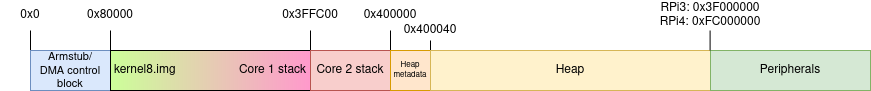
\includegraphics[width=\textwidth]{memorymap.png}
\captionsetup{type=figure}
\caption{Mapa pamięci}
\endgroup
Powyższa ilustracja pokazuje jak wygląda mapa pamięci stworzonego systemu. Może zwrócić uwagę, że pewne elementy zapisywane są zaczynając od adresu 0x0, który tradycyjnie kojarzony jest z nullpointerem, na którym wykonanie jakiejkolwiek operacji zapisu lub odczyty kończy się błędem. W przypadku programowania bare metal tak się jednak nie dziaje. Ponieważ nie ma algorytmów ochrony pamięci, adres 0 traktowany jest tak jak każdy inny. Jest to w pewien sposób problematyczne, ponieważ niektóre błędy, które normalnie byłyby raportowane automatycznie, tutaj są trudniejsze do znalezienia.
\subsection{Sterta i dynamiczna alokacja pamięci}
Alokator pamięci w tym projekcie został zaprojektowany z naciskiem na prostotę i efektywność. Jego konstrukcja opiera się na liście, składającej się z trzech segmentów: headera, payloadu oraz footera. Header i footer zajmują po 4 bajty i przechowują informacje o rozmiarze danego bloku pamięci oraz jego statusie (zaalokowany czy wolny). Natomiast payload to miejsce, w którym przechowywane są faktyczne dane. Dzięki takiej konstrukcji, alokator jest w stanie skutecznie i efektywnie zarządzać przestrzenią pamięci. Co ważne, cała lista znajduje się bezpośrednio w przestrzeni RAM przeznaczonej na stertę, co pozwala na minimalizację zajmowania miejsca na stosie. 
Proces alokacji pamięci w opisywanym systemie przebiega następująco: alokator przeszukuje listę w poszukiwaniu pierwszego bloku o rozmiarze nie mniejszym niż żądany. Gdy odpowiedni blok zostaje zidentyfikowany, dzielony jest on na dwa oddzielne bloki. Pierwszy ma rozmiar zgodny z wymaganiami, natomiast drugi reprezentuje resztę niezaalokowanej pamięci. Po dokonaniu podziału, blok spełniający kryteria jest oznaczany jako zaalokowany, a system zwraca do niego wskaźnik.
Należy podkreślić, że zwracane wskaźniki są wyrównane do 4 bajtów. Jest to procedura niezbędna ze względu na specyfikę architektury procesora RaspberryPi. Wyrównanie dostępu do pamięci do granic 4 bajtów ma krytyczne znaczenie, ponieważ zapewnia optymalne wykorzystanie zasobów procesora. W projektach typu bare-metal niewyrównane dostępy mogą prowadzić do zbędnych cykli procesora, co z kolei wpłynęłoby negatywnie na wydajność całego systemu.
W kontekście zwalniania pamięci, kiedy dany wskaźnik jest uwalniany, odpowiadający mu blok jest oznaczany jako wolny. Alokator następnie sprawdza, czy sąsiednie bloki są również wolne. W przypadku pozytywnej weryfikacji, bloki te są łączone w jeden, co przyczynia się do bardziej efektywnego zarządzania przestrzenią oraz redukcji fragmentacji pamięci.
\subsection{Narzędzia ułatwiające pracę z pamięcią}
Zarządzanie pamięcią w systemach embedded wymaga nie tylko skutecznego alokatora, ale również narzędzi monitorujących i diagnostycznych. Oszczędność miejsca jest kluczowym czynnikiem w środowisku embedded, dlatego każdy niewłaściwie obsłużony fragment pamięci należy wykryć. Aby unikać wycieków pamięci, które mogą poważnie zakłócić działanie systemu i prowadzić do nieprzewidywalnych błędów, wprowadzone zostały różne narzędzia diagnostyczne.
W środowisku programowania embedded, gdzie dostęp do standardowych narzędzi, takich jak Valgrind jest ograniczony, konieczne stało się stworzenie dedykowanych mechanizmów do debugowania. Jednym z takich narzędzi w projekcie jest moduł o nazwie Lickitung. Jego główne zadanie polega na monitorowaniu i weryfikacji procesu zwalniania pamięci. Po zakończeniu sesji, identyfikowanej przez polecenie \texttt{SESSEND}, Lickitung analizuje metadane sterty w poszukiwaniu niezwolnionych bloków. Wykrycie takich bloków skutkuje generowaniem komunikatu o błędzie, informującym o potencjalnym wycieku pamięci, co jest niezwykle pomocne w procesie debugowania.
Dodatkowo, dla celów diagnostycznych, wprowadzona została możliwość wizualizacji struktury pamięci za pomocą instrukcji \texttt{MEM}. Ta funkcjonalność pozwala na wydrukowanie elementów sterty, co znacząco ułatwiało proces identyfikacji potencjalnych problemów z zarządzaniem pamięcią.

\section{MMU}
 Domyślnie procesor wymaga, aby wszystkie dostępy do pamięci miały odpowiednio wyrównany adres. Okazało się to problematyczne, ponieważ w niektórych przypadkach była potrzeba użycia spakowanych struktur (\texttt{\_\_attribute\_\_((\_\_packed\_\_))}). Rozwiązaniem tego problemu jest aktywowanie jednostki zarządzającej pamięcią (\textit{Memory Management Unit, MMU}). Jednak aktywacja MMU niesie za sobą konieczność utworzenia mapy pamięci. Ponieważ projeky ten działa tylko w trybie uprzywilejowanym i nie zachodzi potrzeba tworzenia wielu przestrzeni wirtualnych istnieje tylko jedno mapowanie - jest to proste mapowanie 1:1.

\section{DMA}
Direct Memory Access, znane jako DMA, odgrywa kluczową rolę w zaawansowanych systemach komputerowych, oferując skuteczne mechanizmy przesyłu danych. W opisywanym projekcie, jednym z głównych celów jest zapewnienie użytkownikowi doskonałej jakości interakcji wizualnej. Odbywa się to dzięki modułowi HDMI, którego wydajność jest ściśle związana z mechanizmami przesyłu danych. Aby zoptymalizować ten proces i zapewnić płynność działania, technologia DMA staje się niezbędna. Umożliwia ona bezpośredni transfer ustalonej ilości bajtów między pamięcią a innymi podzespołami sprzętowymi, eliminując potrzebę pośrednictwa procesora.
\subsection{Proces włączenia DMA w Raspberry PI}
Inicjalizacja DMA na platformie Raspberry Pi rozpoczyna się od wyboru odpowiedniego kanału. W ramach realizowanego projektu zdecydowano się na wykorzystanie kanału o nazwie \texttt{DMA\_CHANNEL\_NORMAL}. Po tej operacji następuje konfiguracja transferu, która obejmuje szereg parametrów. Parametry takie jak źródło i cel transferu, rozmiar danych, rodzaj operacji (odczyt czy zapis), wraz z innymi specyfikacjami (ilość danych przeznaczonych do transmisji, prędkość transferu), są ustalane w celu zapewnienia optymalnej funkcjonalności mechanizmu DMA. Dokładna konfiguracja tych parametrów jest niezbędna, aby zagwarantować skuteczność działania mechanizmu DMA.
\subsection{Proces wysyłania danych przez DMA}
Przesyłanie danych za pomocą DMA odbywa się poprzez skonfigurowane kanały, które operują na zdefiniowanych blokach pamięci. W przypadku modułu HDMI, dane graficzne są przesyłane jako sekwencje pikseli. Wprowadzenie DMA do tego procesu umożliwia buforowanie tych danych, a następnie ich sekwencyjne przesyłanie bez ciągłej interakcji z procesorem. Dzięki DMA, przesył danych odbywa się płynnie, z minimalnymi opóźnieniami, co jest szczególnie ważne przy transmisji w czasie rzeczywistym. Wykorzystanie DMA minimalizuje równmież ryzyko wystąpienia błędów transmisji, ponieważ dane są przesyłane w kontrolowanych blokach. Ponadto, znacznie zmniejsza to obciążenie procesora, pozwalając mu na jednoczesne wykonywanie innych, równie istotnych zadań. W efekcie, użytkownik otrzymuje obraz o wysokiej jakości i płynności, co poprawia wrażenia z interakcji z systemem.


\chapter{Komunikacja}
Płytki Raspberry Pi oprócz pokaźnego zestawu pinów GPIO wyprowadzonych na wlutowane w płytkę złącza goldpin posiadają również gotowe porty, takie jak na przykład HDMI, USD czy slot na kartę micro SD, które można wykorzystać do komunikacji z mikro komputerem. Niektóre z dostępnych pinów można skonfigurować tak, by obługiwały pewne popularne protokoły komunikacyjne, takie jak na przykład I2C lub UART. Te rozwiązania znacznie ułatwiają stworzenie insterfejsu do komunikacji człowiek - komputer.

\section{GPIO}
\begingroup
\centering
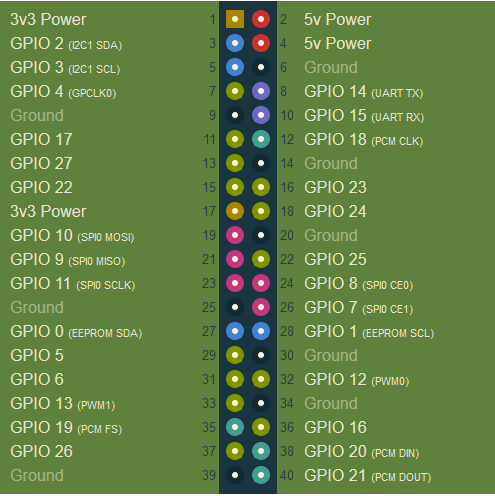
\includegraphics[width=0.5\textwidth]{gpio.png}
\captionsetup{type=figure}
\caption{Piny GPIO na płytce RPi3/RPi4}
\endgroup

W projekcie zaimplementowany został moduł umożliwiający wygodne korzystanie z pinów GPIO. Pozwala on na przełączanie pinów w wybrane tryby, a także odczytywanie i ustawianie stanów na wybranych pinach. Oprócz standardowych trybów \texttt{INPUT} oraz \texttt{OUTPUT} niektóre piny o specjalnym przeznaczeniu mają również tak zwane "funkcje alternatywne" - odpowiadają one za połączenie pinów z wewnętrznymi układami na przykład odpowiedzialnym za komunikację przez specjalne protokoły.

\section{UART}
Najprostszym sposobem na kompunikację z Maliną jest UART. Znany i sprawdzony protokół pozwalający na dwustonną komunikację, w procesie tworzenia projektu sprawdzał się znakomicie jako podstowowe urządzenie wejścia-wyjścia. W celu połączenia z komputerem niezbędny jest konwerter UART-USB.
Raspberry Pi posiada tak naprawdę dwa interfejsy: Mini UART oraz PL011 UART. W tym przypadku konieczne jest skorzystanie z wersji mini, ponieważ to ona ma piny TX oraz RX wyprowadzone na zewnętrzne złącze GPIO, do którego można się podłączyć przewodami. Układ PL011 korzysta z wewnętrznych pinów i jest połączony wewnętrznymi peryferiami, które nie są wykorzystywane w tym projekcie.
Mini UART posiada własne przerwania, a to właśnie na przerwaniach oparty jest system wejścia w tym systemie. Po wejściu do procedury obsługi przerwania z odpowiedniego rejestru odczytywana jest wartość, która została odebrana, a następnie wartość ta wysyłana jest do odpowiedniej funkcji modułu IO, gdzie jest odpowiednio obsługiwana. Jeżeli wartość odpowiada zwykłemu znakowi drukowalnemu, jest wysyłana spowrotem przez UART, aby użytkownik widział co wpisuje. Specjalnej obsługi natomiast wymagają backspace oraz enter. W przypadku tego pierwszego, z bufora danych wejściowych usuwany jest ostatni znak, następnie przez UART wysyłane jest ciąg spacji poprzedzony znakiem \texttt{'\r'} celem wyczyszczenia całej linii i ponownie drukowana jest zawartość bufora. Natomiast obsługa entera sprowadza się do przestawienia flagi \texttt{eol}, która mówi funkcji \texttt{readline()} że może już zwrócić odcztany bufor.
 Korzystanie z UARTa, choć w teorii wystarczające, bo umożliwia komunikacje w obydwie strony, jest o tyle uciążliwe, że wymaga drugiego komputera.

\section{Klawiatura}
Jako samodzielne urządzenie do wprowadzania danych wybór padł na stare klawiatury ze złączem PS/2 lub DIN5. Korzystają one z prostego protokołu wykorzystującego dwa przewody - zegar i dane. Protokół ten jest półdupleksowy, jednak na potrzeby tego projektu dwustronna komunikacja nie jest potrzebna, przyjmowanie danych od klawiatury do Raspberry jest w zupełności wystarczające.

\begingroup
\centering
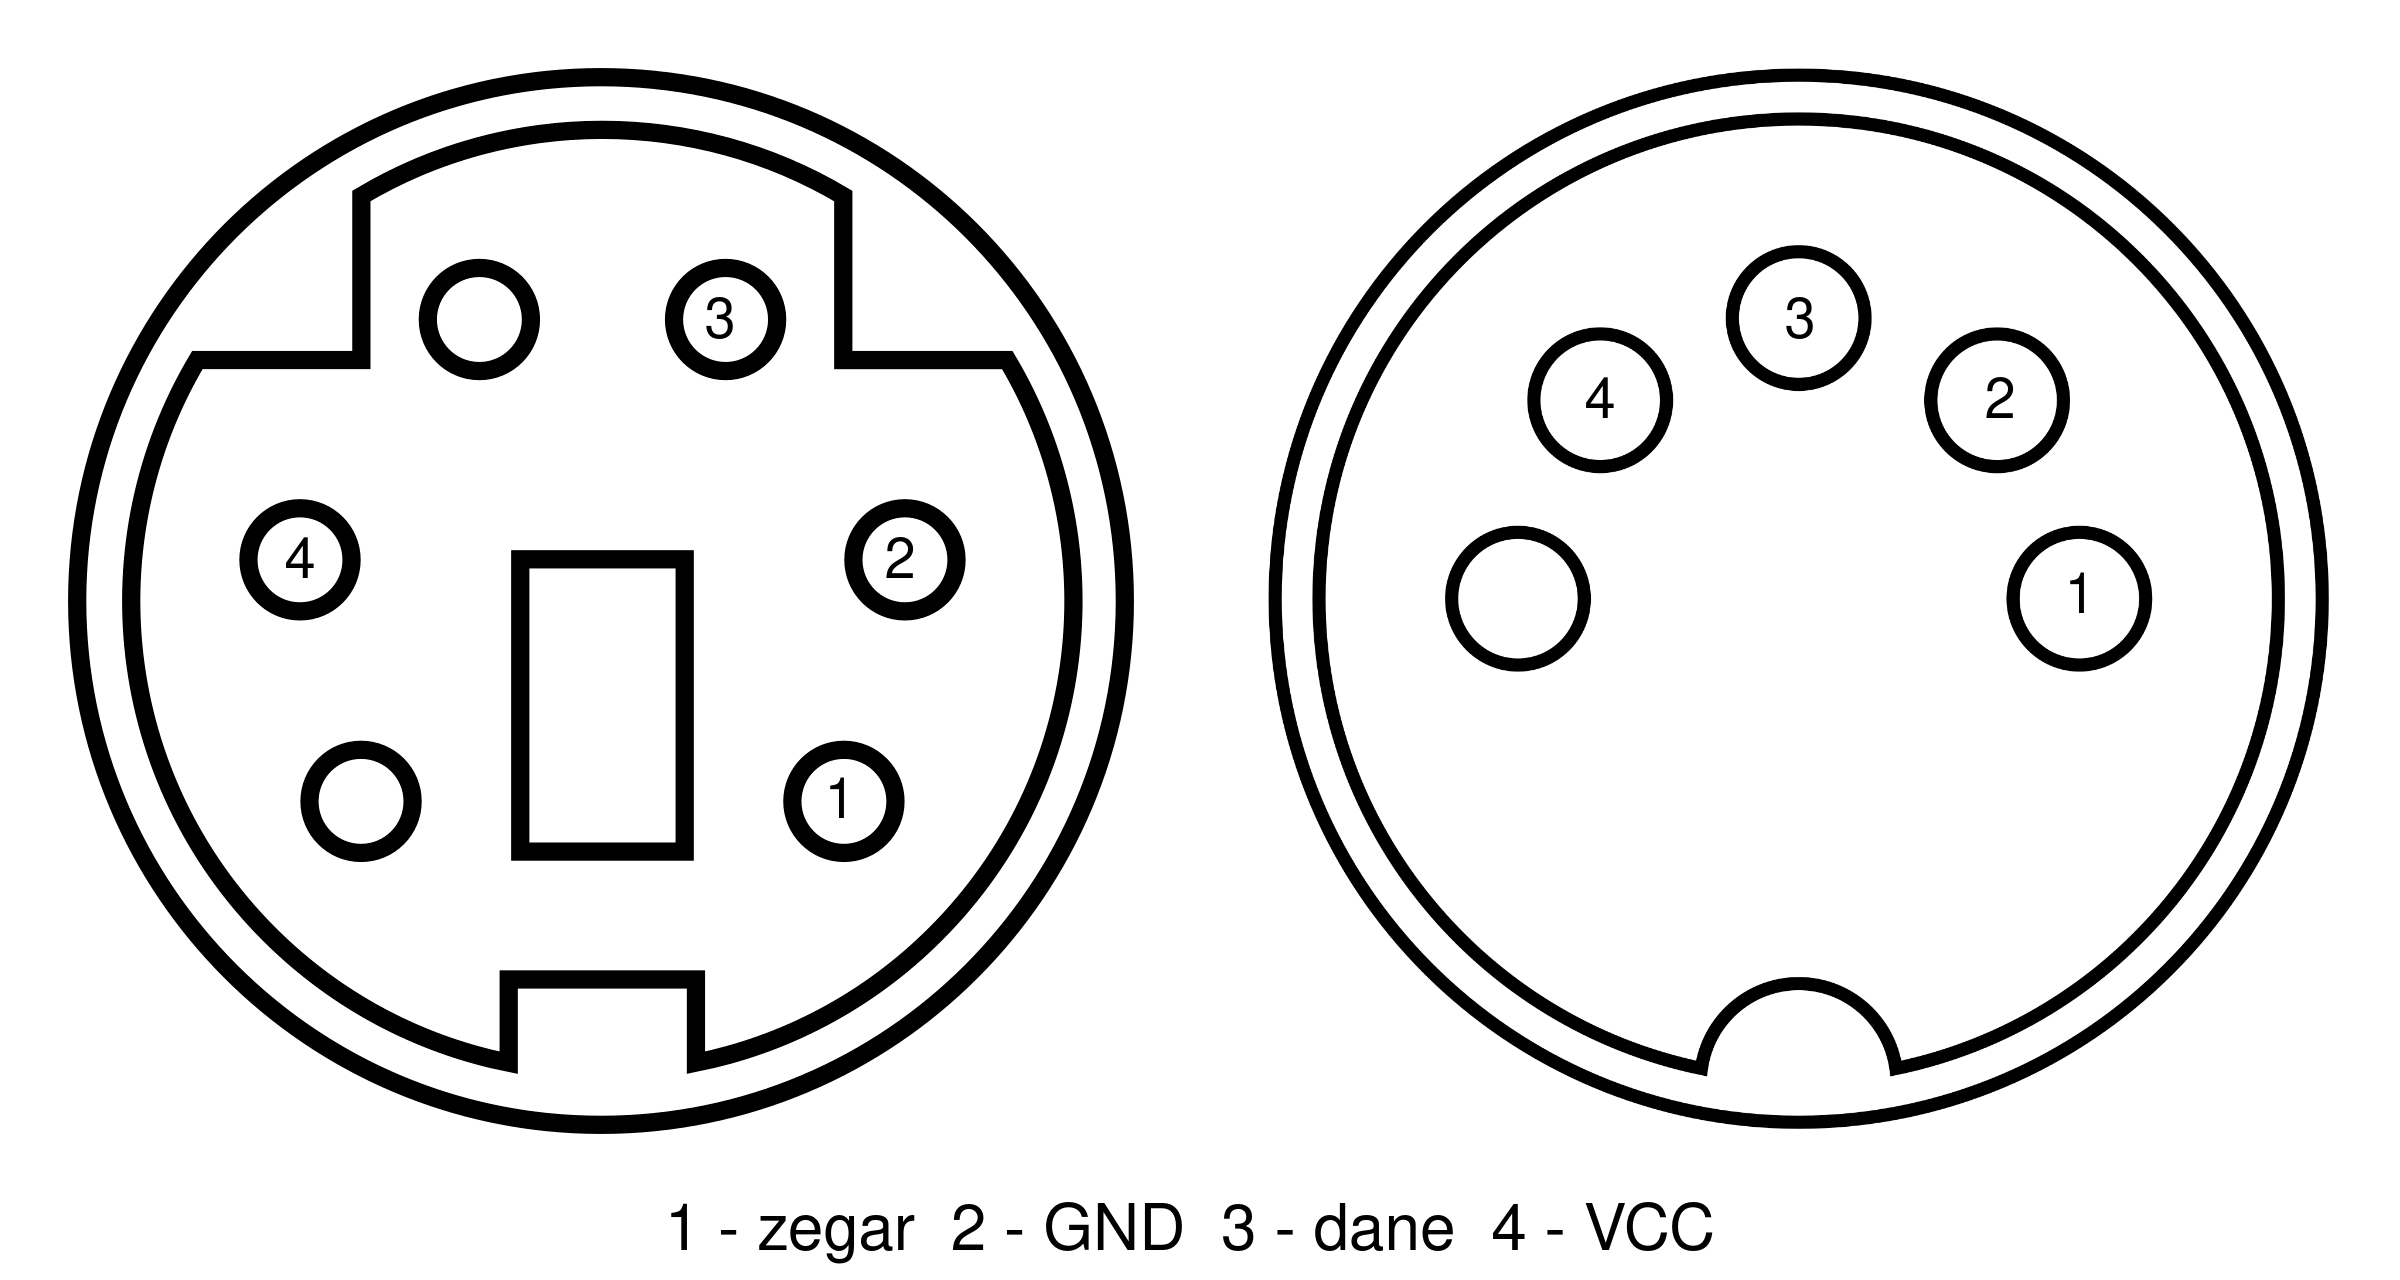
\includegraphics[width=0.75\textwidth]{pinout.png}
\captionsetup{type=figure}
\caption{figure}{Piny męskich złączy PS2 oraz DIN5}
\endgroup

Na jeden kod wysłany przez klawiaturę składa się jedenaście bitów: osiem bitów danych, jeden bit parzystości, oraz po jednym bicie oznaczającym początek oraz koniec transmisji. W celu podłączenie klawiatury do mikrokomputera należy podłączyć przewód danych do pinu nr 5, a przewód zegarowy do pinu nr 6. Na pinie zegarowym włączone jest przerwanie aktywowane zboczem opadającym. Następne w procedurze obsługi przerwania w pętli następuje odczytanie wszystkich 11 bitów, przekonwertowanie na kod ASCII i wysłanie do odpowiedniej funkcji odpowiadającej za obsługę wejścia, tej samej co w przypadku UARTa.

\begingroup
\centering
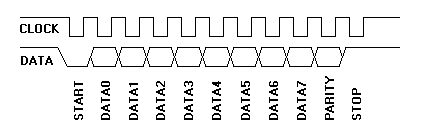
\includegraphics[width=0.75\textwidth]{signals.png}
\captionsetup{type=figure}
\caption{figure}{Sygnały CLOCK oraz DATA}
\endgroup

Wysyłane kody nie są jednak kodami ASCII zrozumiałymi dla języka C, należy je więc najpierw na takie przekonwerować. Oprócz kodów przypisanych do poszczególnych przycisków jest jeszcze specjalny kod o numerze 240, oznaczającymi zwonienie przycisku o kodzie wysłany jako następny. Tak więc na pojedyńcze wciśnięcie klawisza składają się trzy kody: kod wciśniętego przycisku, 240 oraz ponownie kod wciśniętego przyciusku. Dłuższe wciśnięcie jest obsługiwane przez klawiaturę poprzez wielokrotne wysyłanie kodu przycisku przed kodem 240.

\begingroup
\centering
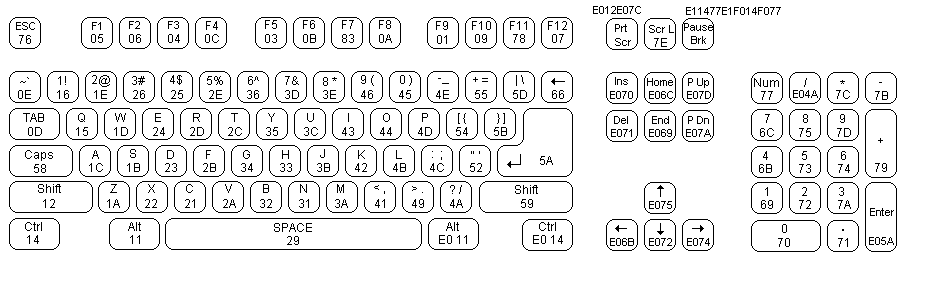
\includegraphics[width=\textwidth]{scancode.png}
\captionsetup{type=figure}
\caption{Kody przycisków na klawiwturze}
\endgroup

Klawiatury standardowo działają z napięciem zasilania +5V i takie też napięcie wysyłają na piny danych i zegara. Piny GPIO działają natomiast z napięciem +V. Niektóre klawiatury działają z niższym napięciem, jednak by mieć pewność, że każda klawiatura będzie działać prawidłowo, w projekcie wykorzystany został prosty konwerter poziomów logicznych bazujący na układzie BSS138.
 
\section{HDMI}
W ramach rozwoju przedstawionego systemu, kluczowym wyzwaniem stało się umożliwienie użytkownikowi wizualnej interakcji z interfejsem. W tym celu niezbędne okazało się zaprojektowanie i wdrożenie dedykowanego modułu HDMI, który odpowiedzialny jest za przesyłanie obrazu do urządzenia wyświetlającego.
\subsection{Inicjalizacja i konfiguracja HDMI}
Inicjalizacja HDMI w Raspberry Pi rozpoczyna się od aktywacji VideoCore za pośrednictwem mechanizmu Mailbox. Mailbox to specyficzny mechanizm komunikacyjny służący do wymiany wiadomości między głównym procesorem a procesorem VideoCore. Dzięki temu rozwiązaniu możliwa jest dwukierunkowa komunikacja, co umożliwia głównemu procesorowi wysyłanie żądań konfiguracyjnych i otrzymywanie odpowiedzi od VideoCore, dedykowanej jednostki graficznej odpowiadającej za wiele operacji sprzętowych, w tym zarządzaniem sygnałami wideo.
Następnie przeprowadzana jest konfiguracja modułu HDMI. Dla potrzeb projektu wybrano rozdzielczość 640x400 pikseli, nawiązując w ten sposób do proporcji charakterystycznych dla komputerów typu Commodore 64. Parametr "bits per pixel", ustalony na wartość 32, oznacza liczbę bitów używanych do reprezentowania koloru pojedynczego piksela (format RGBA). Ustawienie wartości w ten sposób umożliwia precyzyjne odwzorowanie szerokiej gamy kolorów, co przekłada się na wysoką jakość wyświetlanego obrazu.
\subsection{Aktualizacja bufora i wydajność}
Aby uzyskać odpowiednią jakość wyświetlanego obrazu, kluczowe jest efektywne aktualizowanie ekranu. Proces ten polega na sekwencyjnym przypisywaniu wartości kolorów w formie 32-bitowych liczb reprezentujących poszczególne piksele. Chociaż taka metoda wydaje się prosta, napotyka pewne wyzwania techniczne. Sekwencyjne pisanie każdego piksela bezpośrednio pod wskaźnik bufora ramki może prowadzić do znaczących opóźnień, zwłaszcza gdy konieczne jest odświeżenie całego ekranu. Wynika to z konieczności przetwarzania każdej operacji zapisu oraz komunikacji z pamięcią RAM przez procesor, co wprowadza dodatkowe opóźnienia. Optymalne rozwiązanie tego problemu polega na zastosowaniu opisanej wcześniej technologii DMA.
Dodatkowo, dla zwiększenia funkcjonalności, zaimplementowano możliwość scrollowania ekranu w dół. Aby osiągnąć ten efekt, zastosowano bufor cykliczny. Dodatkowo zapamiętywany jest indeks piksela, który służy jako punkt odniesienia do określenia, które dane mają być wyświetlane na początku ekranu podczas przewijania. Bufor cykliczny jest następnie przetwarzany w odpowiedniej kolejności dzięki technologii DMA, tworząc dla użytkownika iluzję ciągłego, nieskończonego przewijania ekranu.

\section{Karta SD}
Konieczność pisania nowych programów z każdym uruchomieniem komputera byłaby bardzo uciążliwa, dlatego system wspiera zapisywanie stworzonych programów w zewnętrznej pamięci nieulotnej. Do tego celu wykorzystana została ta sama karta SD, z której ładowany jest program. Aby rozwiązanie zadziałało na karcie prócz partycji niezbędnej do bootowania płytki musi zostać utworzona druga partycja o dowolnym typie, ponieważ dane przechowywane będą we własnościowym formacie. 
\subsection{Komunikacja z kartą SD}
Do komunikacji procesora z kartą posłuży wbudowany w płytkę kontroler zewnętrznej pamięci masowej (\textit{.: External Mass Media Controller, EMMC}). Aby z niego skorzystać, należy najpierw odpowiednio skonfigurować wykorzystywane piny GPIO: piny 34-39 jako \texttt{INPUT} oraz piny 48-52 jako funkcję \texttt{ALT3}. Komunikacja odbywa się za pomocą zestawu rejestrów oraz specjalnych komend wysyłanych przez te rejestry. Podstawowymi komendami są komendy nr 17 oraz 24, odpowiedzialne za odpowiednio odczyt oraz zapis bloku (512MB), a także komenda 0, która resetuje kartę i od której rozpoczyna się cała komunikacja.
Poniższy diagram przedstawia proces łączenia się z kartą SD i transfery danych:

\begingroup
\centering
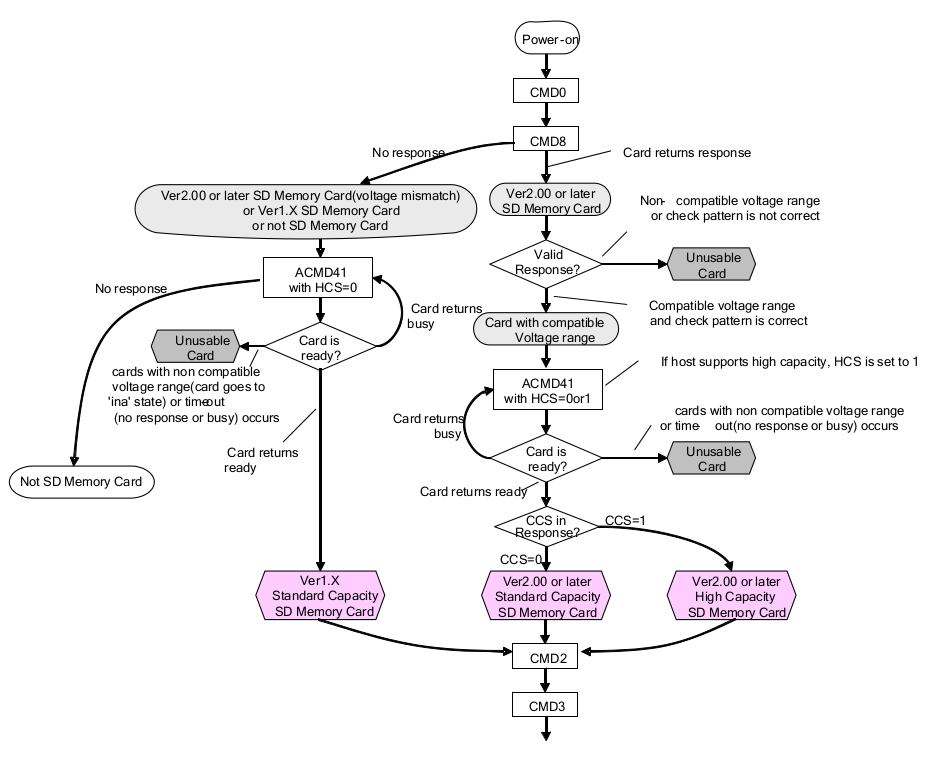
\includegraphics[width=\textwidth]{sd-connection.png}
\captionsetup{type=figure}
\caption{Inicjalizacja i połączenie z kartą SD}
\endgroup

\begingroup
\centering
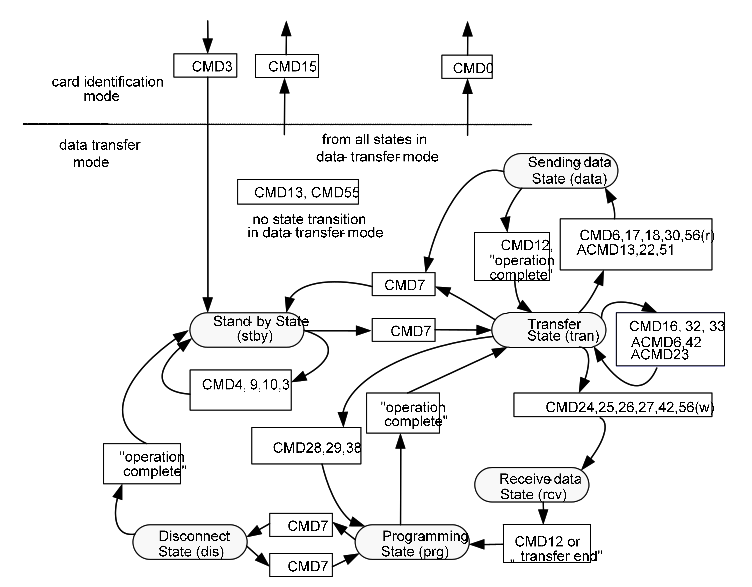
\includegraphics[width=\textwidth]{sd-transfer.png}
\captionsetup{type=figure}
\caption{Zapis i odczyt}
\endgroup

\subsection{Przechowywanie danych}
Program nie wspiera żadnego ze standardowych systemów plików, a dane przechowuje we własnościowym formacie. Po włączeniu mikrokomputera nastąpi próba inicjalizacji systemu plików. Za partycję danych posłuży pierwsza (po partycji z systemem) partycja znaleziona w głównym rekordzie rozruchowym (textit{.: Master Boot Record, MBR}), której rozmiar będzie wynosił przynajmniej 1 gigabajt. Pierszy blok partycji danych przechowywał będzie tablicę plików, której pojedyńczy element stanowi następująca struktura:
\begin{verbatim}
#define FILENAME_LEN 10

typedef struct {
  u32 size_in_bytes;
  u8 id;
  u8 type;
  char name[FILENAME_LEN];
} fileS;
\end{verbatim}

Isnienie pliku w danym miejscu w tablicy wskazuje pole \texttt{type} - jeżeli jest różne od zera, plik istnieje. Póki co wspierane jest jedynie zapisywanie programów w BASICU, więc 8 bitów jest trochę na wyrost, ale jest to furtka na przyszłość do przechowywania w pamięci nieulotnej na przykład całych sesji lub obrazków. Tablica przechowuje dane o 32 plikach. Cała partycja danych dzielona jest na równe kawałki, które kolejno przyporządkowane są wpisom w tablicy plików. Pierwszy wpis jest specjalny i sygnalizuje systemowi istnienie całego systemu plików: jeżeli po wczytaniu pierwszego bloku partycji danych odnaleziony zostanie tam wpis o \texttt{id} równym 0, \texttt{type} równym 105 oraz nazwie \texttt{"SPECIAL"}, program potraktuje pierwszy blok jako gotową tablicę plików. W przeciwnym wypadku taka tablica zostanie utworzona.
\subsection{Obsługa plików}
Do korzystania z systemu plików udostępnione zostały następujące komendy: 
\begin{itemize}
 \item \texttt{LS} - wypisuje wszystkie pliki zapisane na karcie SD
 \item \texttt{SAVE name} - zapisuje program z aktualnej sesji do pliku z podaną nazwą
 \item \texttt{LOAD name} - ładuje program o podanej nazwie z kadty SD do adkutalnej sesji
 \item \texttt{DELETE name} - usuwa podany program z karty SD
\end{itemize}
W każdej z podanych komend \texttt{name} musi być różne od \texttt{"SPECIAL"} i może mieć co najwyżej 10 znaków


\chapter{Podsumowanie}
Realizacja projektu polegającego na stworzeniu systemu bare-metal dla platformy Raspberry Pi z interpreterem języka BASIC była nie tylko ambitnym przedsięwzięciem, ale również źródłem wielu wyzwań oraz okazją do zdobycia cennych doświadczeń. Podczas pracy nad projektem niejednokrotnie napotykano na różnego rodzaju trudności i przeszkody, które wymagały nie tylko kreatywnego myślenia, ale także głębszego zrozumienia złożonych koncepcji informatycznych.
Prace nad takim projektem dają możliwość pogłębienia wiedzy w wielu obszarach informatyki. W tym przypadku, zdobyto doświadczenie z zakresu programowania embedded, zrozumiano głębsze aspekty działania systemów oraz mechanizmów stojących za interpreterami. Znaczący rozmiar projektu pozwolił również na naukę efektywnego zarządzania dużą ilością kodu oraz organizacji pracy w dwuosobowym zespole.
Rezultat prezentowanej pracy nie tylko demonstruje efektywne wdrożenie założonych celów, ale również otwiera pole do przyszłej dalszej rozbudowy zaprojektowanego systemu. 
%%%%% BIBLIOGRAFIA

\begin{thebibliography}{1}

\bibitem{} Raspberry Pi documentation\\(\url{https://www.raspberrypi.com/documentation/})
\bibitem{} BCM 2837 datasheet (RPi3)\\(\url{https://datasheets.raspberrypi.com/bcm2835/bcm2835-peripherals.pdf})
\bibitem{} BCM 2711 datasheet (RPi4)\\(\url{https://datasheets.raspberrypi.com/bcm2711/bcm2711-peripherals.pdf})
\bibitem{} 101 BASIC computer games\\(\url{https://annarchive.com/files/Basic_Computer_Games_Microcomputer_Edition.pdf})
\bibitem{} Low Level Devel (\url{https://github.com/rockytriton/LLD/tree/main})
\bibitem{} uBASIC: a really simple BASIC interpreter\\ (\url{https://github.com/adamdunkels/ubasic})
\bibitem{} SD and SDIO (\url{http://yannik520.github.io/sdio.html})
\bibitem{} Bare Metal RPi4OS (\url{https://www.rpi4os.com/})
\bibitem{} Czcionka (\url{https://github.com/dhepper/font8x8})
\bibitem{} Mikrokomputery: Commodore 64 ~ Bohdan Frelek

\end{thebibliography}

\end{document}